\documentclass[10pt,landscape,a4paper]{article}
\usepackage{multicol}
\usepackage{ifthen}
\usepackage[landscape]{geometry}
\usepackage[dvipsnames]{xcolor}
\usepackage{hyperref}
\hypersetup{colorlinks=true}

% Math symbols
\usepackage{amsmath}

% Tikz
\usepackage{tikz}
\usetikzlibrary{decorations.pathreplacing,decorations.markings,calc}
\tikzset{
  % style to apply some styles to each segment of a path
  on each segment/.style={
    decorate,
    decoration={
      show path construction,
      moveto code={},
      lineto code={
        \path [#1]
        (\tikzinputsegmentfirst) -- (\tikzinputsegmentlast);
      },
      curveto code={
        \path [#1] (\tikzinputsegmentfirst)
        .. controls
        (\tikzinputsegmentsupporta) and (\tikzinputsegmentsupportb)
        ..
        (\tikzinputsegmentlast);
      },
      closepath code={
        \path [#1]
        (\tikzinputsegmentfirst) -- (\tikzinputsegmentlast);
      },
    },
  },
  % style to add an arrow in the middle of a path
  direct arrow/.style={postaction={decorate,decoration={
        markings,
        mark=at position .8 with {\arrow[>=stealth]{>}}
      }}},
  % style to add an arrow in the middle of a path
  reverse arrow/.style={postaction={decorate,decoration={
        markings,
        mark=at position .8 with {\arrow[>=stealth]{<}}
      }}},
}

% Narrow margins
\ifthenelse{\lengthtest { \paperwidth = 11in}}
	{ \geometry{top=.5in,left=.5in,right=.5in,bottom=.5in} }
	{\ifthenelse{ \lengthtest{ \paperwidth = 297mm}}
		{\geometry{top=1cm,left=1cm,right=1cm,bottom=1cm} }
		{\geometry{top=1cm,left=1cm,right=1cm,bottom=1cm} }
	}

% Turn off header and footer
\pagestyle{empty}

% Redefine section commands to use less space
\makeatletter
\renewcommand{\section}{\@startsection{section}{1}{0mm}%
                                {-1ex plus -.5ex minus -.2ex}%
                                {0.5ex plus .2ex}%x
                                {\normalfont\large\bfseries\center\color{Red}}
}
\renewcommand{\subsection}{\@startsection{subsection}{2}{0mm}%
                                {-1explus -.5ex minus -.2ex}%
                                {0.5ex plus .2ex}%
                                {\normalfont\normalsize\bfseries\center\color{RoyalBlue}}
}
\makeatother

% Don't print section numbers
\setcounter{secnumdepth}{0}


% Helper commands to format PDF commands specs
\newcommand{\pdfopnoit}[3]{\texttt{#2} & {#1} & {#3} \\}
\newcommand{\pdfop}[3]{\pdfopnoit{\it #1}{#2}{#3}}


% -----------------------------------------------------------------------

\begin{document}

\raggedright
\begin{multicols}{3}

% multicol parameters
% These lengths are set only within the two main columns
%\setlength{\columnseprule}{0.25pt}
\setlength{\premulticols}{1pt}
\setlength{\postmulticols}{1pt}
\setlength{\multicolsep}{1pt}
\setlength{\columnsep}{2pt}

\begin{center}
\Large \textbf{\color{Green}{PDF Graphic Operators}} \\
\normalsize by Guillaume Endignoux \\
\url{https://gendignoux.com}
\end{center}

% -----------------------------------------------------------------------

\section{Definitions}

\subsection{Postfix notation}
\begin{tabular}{@{}lll@{} }
\pdfop{foo bar}{op}{$\rightarrow$ written in file as ``\texttt{foo bar op}''}
\end{tabular}

\subsection{Filling rules}
\begin{center}
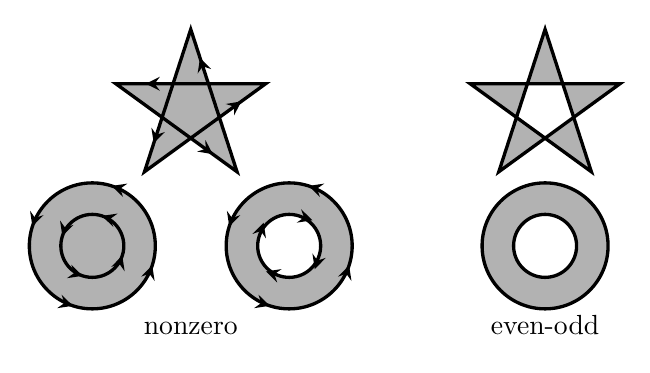
\begin{tikzpicture}

% Stars
\foreach \a in {90, 162, 234, 306, 18} {
    \coordinate (p1) at (\a:1);
    \coordinate (p2) at (\a+72:1);
    \coordinate (p3) at (\a+144:1);
    \coordinate (p4) at (\a+216:1);
    \coordinate (p5) at (\a+288:1);

    \coordinate (t1) at (intersection of p1--p3 and p2--p4);
    \coordinate (t2) at (intersection of p1--p3 and p2--p5);

    \fill[color=black!30] ($(p2) + (4.5,0)$) -- ($(t1) + (4.5,0)$) -- ($(t2) + (4.5,0)$) -- cycle;
}

\fill[color=black!30] (90:1) -- (234:1) -- (18:1) -- (162:1) -- (306:1) -- cycle;

\draw[very thick, postaction={on each segment={direct arrow}}] (90:1) -- (234:1) -- (18:1) -- (162:1) -- (306:1) -- cycle;
\draw[very thick] ($(90:1) + (4.5,0)$) -- ($(234:1) + (4.5,0)$) -- ($(18:1) + (4.5,0)$) -- ($(162:1) + (4.5,0)$) -- ($(306:1) + (4.5,0)$) -- cycle;

% Circles
\fill[color=black!30] (-1.25, -1.75) circle (0.8);
\fill[color=black!30, even odd rule] (1.25, -1.75) circle (0.8) (1.25, -1.75) circle (0.4);
\fill[color=black!30, even odd rule] (4.5, -1.75) circle (0.8) (4.5, -1.75) circle (0.4);

\draw[very thick, postaction={on each segment={direct arrow}}] (-1.25, -1.75) circle (0.8);
\draw[very thick, postaction={on each segment={direct arrow}}] (-1.25, -1.75) circle (0.4);
\draw[very thick, postaction={on each segment={direct arrow}}] (1.25, -1.75) circle (0.8);
\draw[very thick, postaction={on each segment={reverse arrow}}] (1.25, -1.75) circle (0.4);
\draw[very thick] (4.5, -1.75) circle (0.4);
\draw[very thick] (4.5, -1.75) circle (0.8);

% Caption
\draw (0, -3) node[anchor=south] {nonzero};
\draw (4.5, -3) node[anchor=south] {even-odd};

\end{tikzpicture}


\end{center}

\subsection{Matrix}
\begin{center}
\textit{a b c d e f} $\mapsto \begin{pmatrix}
a & b & 0 \\
c & d & 0 \\
e & f & 1
\end{pmatrix}$
\end{center}


\section{Graphic state}

\subsection{General}
\begin{tabular}{@{}lll@{} }
\pdfop{lineWidth}{w}{set line width}
\pdfop{lineCap}{J}{set cap style}
\pdfop{lineJoin}{j}{set join style}
\pdfop{miterLimit}{M}{set miter limit}
\pdfop{dashArray dashPhase}{d}{set dash pattern}
\pdfop{intent}{ri}{set color rendering intent}
\pdfop{flatness}{i}{set flatness tolerance}
\pdfop{dictName}{gs}{set graphic state parameters}
\end{tabular}

\subsection{Special}
\begin{tabular}{@{}lll@{} }
\pdfop{}{q}{save state}
\pdfop{}{Q}{restore state}
\pdfop{a b c d e f}{cm}{set transformation matrix}
\end{tabular}


\section{Images}

\begin{tabular}{@{}lll@{} }
\pdfop{name}{Do}{paint XObject}
\pdfop{}{BI}{begin inline image}
\pdfop{}{ID}{begin inline image data}
\pdfop{}{EI}{end inline image}
\end{tabular}


\section{Path}

\subsection{Construction}
\begin{tabular}{@{}lll@{} }
\pdfop{x y}{m}{move to}
\pdfop{x y}{l}{line to}
\pdfop{$x_1$ $y_1$ $x_2$ $y_2$ $x_3$ $y_3$}{c}{cubic B\'{e}zier to}
\pdfop{$x_2$ $y_2$ $x_3$ $y_3$}{v}{B\'{e}zier with $(x_1, y_1)$ = current}
\pdfop{$x_1$ $y_1$ $x_3$ $y_3$}{y}{B\'{e}zier with $(x_2, y_2) = (x_3, y_3)$}
\pdfop{}{h}{close path}
\pdfop{x y width height}{re}{rectangle with $(x, y)$ = low-left}
\end{tabular}

\subsection{Clipping}
\begin{tabular}{@{}lll@{} }
\pdfop{}{W}{intersect + set clipping (nonzero rule)}
\pdfop{}{W*}{intersect + set clipping (even-odd rule)}
\end{tabular}

\subsection{Painting}
\begin{tabular}{@{}lll@{} }
\pdfop{}{S}{stroke}
\pdfop{}{s}{close + stroke}
\pdfop{}{f}{fill (nonzero rule)}
\pdfop{}{F}{deprecated, same as \texttt{f}}
\pdfop{}{f*}{fill (even-odd rule)}
\pdfop{}{B}{fill + stroke (nonzero rule)}
\pdfop{}{B*}{fill + stroke (even-odd rule)}
\pdfop{}{b}{close + fill + stroke (nonzero rule)}
\pdfop{}{b*}{close + fill + stroke (even-odd rule)}
\pdfop{}{n}{end path (no-op)}
\end{tabular}


\section{Text}

\subsection{Objects}
\begin{tabular}{@{}lll@{} }
\pdfop{}{BT}{begin text}
\pdfop{}{ET}{end text}
\end{tabular}

\subsection{State}
\begin{tabular}{@{}lll@{} }
\pdfop{charSpace}{Tc}{set char spacing}
\pdfop{wordSpace}{Tw}{set word spacing}
\pdfop{scale}{Tz}{set horiz. scaling (in percent)}
\pdfop{leading}{TL}{set text leading}
\pdfop{font size}{Tf}{set font + size}
\pdfop{render}{Tr}{set text rendering mode}
\pdfop{rise}{Ts}{set text rise}
\end{tabular}

\subsection{Positioning}
\begin{tabular}{@{}lll@{} }
\pdfop{$t_x$ $t_y$}{Td}{next line (w.r.t start of current line)}
\pdfop{$t_x$ $t_y$}{TD}{next line + set text leading}
\pdfop{a b c d e f}{Tm}{set text matrix}
\pdfop{}{T*}{next line}
\end{tabular}

\subsection{Showing}
\begin{tabular}{@{}lll@{} }
\pdfop{string}{Tj}{show string}
\pdfop{string}{'}{next line + show string}
\pdfop{$a_w$ $a_c$ string}{"}{set spacings + next line + show}
\pdfop{array}{TJ}{show strings (+ manual spacing)}
\end{tabular}


\section{Color}

\subsection{Stroking}

\begin{tabular}{@{}lll@{} }
\pdfop{name}{CS}{set color space}
\pdfop{$c_1 ... c_n$}{SC}{set color}
\pdfopnoit{$c_1 ... c_n$ [\textit{name}]}{SCN}{set color}
\pdfop{gray}{G}{set gray color}
\pdfop{r g b}{RG}{set RGB color}
\pdfop{c m y k}{K}{set CMYK color}
\end{tabular}

\subsection{Non-stroking}

Same operators as stroking but in \texttt{lowercase}.


\section{Misc}

\subsection{Type 3 fonts}
\begin{tabular}{@{}lll@{} }
\pdfop{$w_x$ $w_y$}{d0}{glyph width}
\pdfop{$w_x$ $w_y$ $ll_x$ $ll_y$ $ur_x$ $ur_y$}{d1}{width + bounding box}
\end{tabular}

\subsection{Marked content}
\begin{tabular}{@{}lll@{} }
\pdfop{tag}{MP}{marked-content point}
\pdfop{tag props}{DP}{point with properties}
\pdfop{tag}{BMC}{begin marked-content sequence}
\pdfop{tag props}{BDC}{begin sequence with properties}
\pdfop{}{EMC}{end marked-content sequence}
\end{tabular}

\subsection{Other}
\begin{tabular}{@{}lll@{} }
\pdfop{name}{sh}{paint shading to clipping path}
\pdfop{}{BX}{begin compatibility section}
\pdfop{}{EX}{end compatibility section}
\end{tabular}


% -----------------------------------------------------------------------

\begin{center}
\rule{0.3\linewidth}{0.25pt}
\end{center}


\includegraphics[width=6em]{figures/by_nc_sa.eps}
This work is licensed under a \href{http://creativecommons.org/licenses/by-nc-sa/4.0/}{Creative Commons Attribution-NonCommercial-ShareAlike 4.0 International License}.

\copyright{} 2016 Guillaume Endignoux.

Source: \url{https://github.com/gendx/pdf-cheat-sheets}.

Based on \LaTeX{} templates by \href{http://www.stdout.org/~winston/latex/}{Winston Chang} and \href{https://github.com/adamatan/Cheat-Sheets}{Adam Matan}.

\end{multicols}
\end{document}

